\documentclass[12pt, letterpaper]{article}
\usepackage[utf8]{inputenc}
\usepackage{graphicx}
\author{
Universidad Autónoma de Nuevo León \\
Facultad de Ingeniería Mecánica y Eléctrica \\
\\
Diego Iván Garza Tristán\\
1678477
\\
\and
Moisés de Jesús Gálvez Rivera\\
1791853
\and
Andrea Amador Burgueño\\
1791890
\and
Sergio Andrés Muñoz Pinedo\\
1669194
\\[3ex]
César Javier Martinez Vazquez\\
1586241
}

\title{C3: Robot solucionador de cubos de Rubik.}
\date{19 de Mayo 2017}

\begin{document}
\maketitle
\pagenumbering{gobble}
\newpage
\tableofcontents
\newpage
\pagenumbering{arabic}
\begin{abstract}
Construcción de un robot/máquina que resuelve cubos de Rubik 3x3x3 mediante el método de Kociemba, escrito en Arduino y Python.
\end{abstract}

\section{Introducción.}
\subsection{Historia del cubo de Rubik.}
\paragraph{}
A mediados de la década de 1970, Ernő Rubik trabajaba en el Departamento de Diseño de Interiores en la Academia de Artes y Trabajos Manuales Aplicados en Budapest. Aunque generalmente se dice que el cubo fue construido como herramienta escolar para ayudar a sus estudiantes a entender objetos tridimensionales, su propósito real era resolver el problema estructural que lograra mover las partes independientemente sin que el mecanismo entero se desmoronara. Rubik no se dio cuenta de que había creado un rompecabezas hasta la primera vez que mezcló su nuevo cubo e intentó volverlo a la posición original. Obtuvo una patente húngara (HU170062) en 1975. Originalmente, el cubo de Rubik fue llamado Cubo Mágico (Bűvös kocka) en Hungría. El rompecabezas no había sido patentado internacionalmente en el plazo de un año de la patente original. De esta manera, la ley de patentes impedía la posibilidad de patentarlo a nivel internacional. Ideal quería al menos un nombre reconocible para registrar; el acuerdo puso a Rubik en el centro de atención debido a que el cubo mágico fue renombrado como su inventor.

\begin{figure}[hb]
	\centering
	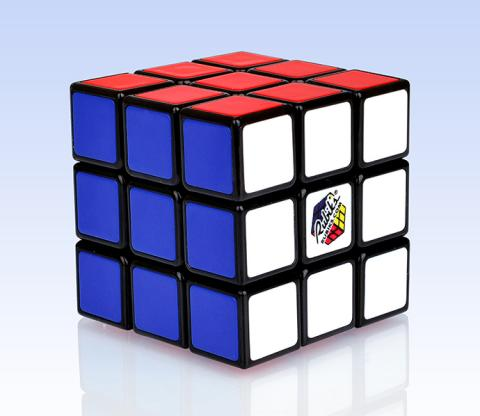
\includegraphics[scale=0.4]{images/rubiks.jpg}
	\caption{Cubo de Rubik resuelto.}
	\label{fig:rubiks}
\end{figure}
\paragraph{}
Los primeros productos de este invento salieron a la venta a finales de 1977 en jugueterías de Budapest. El cubo mágico se unía por medio de piezas de plástico ensambladas entre sí que prevenían que las piezas se separaran, a diferencia de los imanes en el diseño de Nichols. En septiembre de 1979 se firmó un acuerdo con Ideal para vender el cubo mágico a nivel mundial y el rompecabezas hizo su debut internacional en ferias de juguetes de Londres, París, Nürnberg y Nueva York en enero y febrero de 1980.
\paragraph{}
Después del éxito internacional del Cubo Rubik en las jugueterías occidentales se detuvo brevemente para que el juguete pudiera adecuarse a los estándares occidentales de seguridad y empaquetado. Se produjo un cubo más ligero e Ideal, Toys decidió cambiarle el nombre; se consideraron "El nudo gordiano" y "Oro Inca", pero la compañía finalmente se decidió por "El cubo de Rubik", la primera entrega fue exportada de Hungría en mayo de 1980. A raíz de la escasez del producto surgieron muchas imitaciones más baratas.
\subsection{Mecanismo del cubo.}
\paragraph{}
Un cubo de Rubik estándar mide 5.7 cm por lado, aunque existen variaciones. El rompecabezas consta de 26 piezas o cubos pequeños. Cada una incluye una extensión interna oculta que se entrelaza con los otros cubos, mientras les permite moversa a diferentes posiciones. Sin embargo, las piezas centrales de cada una de las seis caras son simplemente un cuadro fijado al mecanismo principal. Esto provee la estructura para que las otras piezas quepan y giren alrededor.
\begin{figure}[hb]
	\centering
	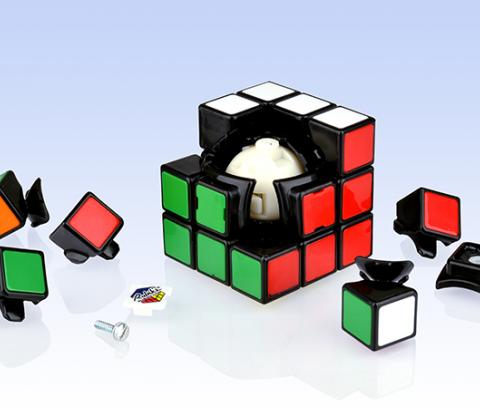
\includegraphics[scale=0.4]{images/mechanism.jpg}
	\caption{Un cubo de Rubik semi ensamblado}
	\label{fig:mechanism}
\end{figure}
\paragraph{}
Cada uno de los seis centros gira en un tornillo sujetado por la pieza central. Un resolte entre cada cabeza de tornillo y su correspondiente pieza tensiona la pieza hacia el interior, por lo que el conjunto se mantiene compacto, pero todavía se puede manipular fácilmente. El tornillo se puede apretar o aflojar para cambiar la tensión del cubo. 
\paragraph{}
Hay seis piezas centrales que muestran una cara de un solo color, doce piezas arista que muestran dos caras coloreadas, y ocho piezas vértice que muestran tres caras coloreadas. Cada pieza muestra una combinación única de colores, pero no todas las combinaciones están presentes, por ejemplo, si rojo y naranja son lados opuestos de un cubo resuelto, no habrá pieza arista roja-naranja. En un cubo de Rubik estándar se encuentran seis colores: blanco, amarillo, naranja, rojo, verde y azul. En la figura \ref{fig:stickers} se muestra la configuración estándar de dichos colores.
\begin{figure}[hb]
	\centering
	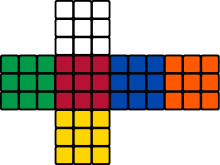
\includegraphics[scale=0.5]{images/stickers.png}
	\caption{Colores en el cubo}
	\label{fig:stickers}
\end{figure}
\subsection{Variaciones.}
\paragraph{}
Existen diferentes variaciones del cubo de Rubik, de la familia NxN desde N=2 hasta N=22 donde todos son cubos, los NxNxN que suelen ser modificaciones, son cubos que pueden llegar a tener diferente número de piezas por piezas por lado como por ejemplo 3x4x5 que significa 3 piezas ancho, 4 piezas alto y 5 piezas de largo. También existe la familia Minx, que incluye varias formas diferentes al cubo siendo las más comunes las pirámides y dodecaedros. Los cubos más conocidos de esta familia son el Pyraminx, una pirámide que gira 120 grados por cada cara, y el Megaminx que es un dodecaedro que gira 72 grados por cara.
\begin{figure}[ht]
   \begin{minipage}{0.48\textwidth}
     \centering
     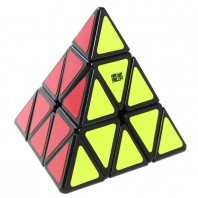
\includegraphics[width=.7\linewidth]{images/pyraminx.jpg}
     \caption{MoYu Pyraminx}\label{Fig:pyraminx}
   \end{minipage}\hfill
   \begin {minipage}{0.48\textwidth}
     \centering
     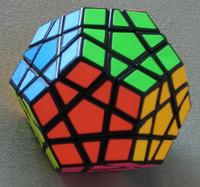
\includegraphics[width=.7\linewidth]{images/megaminx.jpg}
     \caption{Megaminx}\label{Fig:megaminx}
   \end{minipage}		
\end{figure}

\subsection{Algoritmos de solución.}
\subsection*{Notación.}
\paragraph{}
La notación más usual es la desarrollada por David Singmaster usada para denotar la secuencia de movientos, denominada "notación Singmaster". Su naturaleza relativa permite que los algoritmos se escriban de manera tal que puedan aplicarse independientemente de a qué lado es designado el superior o cómo están organizados los colores en un cubo particular, la notación proviene de la inicial del nombre de la cara, es decir ``F" significaría \emph{``front"}, ``B" sería \emph{``back"}, entre otros.
\begin{itemize}
	\item \emph{R (derecha)}: el lado directamente a la derecha del frente
	\item \emph{L (izquierda)}: el lado directamente a la izquierda del frente.
	\item \emph{U (arriba)}: el lado encima o en la parte superior del lado frontal.
	\item \emph{D (abajo)}: el lado opuesto a la parte superior, debajo del cubo.
	\item \emph{F (frente)}: el lado enfrente a la persona.
	\item \emph{B (atrás)}: el lado opuesto al frente.
	\item \emph{Rw}: el lado a la derecha del frente y la correspondiente capa media.
	\item \emph{Lw}: el lado a la izquierda del frente y la correspondiente capa media.
	\item \emph{Uw}: el lado superior y la correspondiente capa media.
	\item \emph{Dw}: el lado inferior y la correspondiente capa media.
	\item \emph{Fw}: el lado enfrente a la persona y la correspondiente capa media.
	\item \emph{Bw}: el lado opuesto al frente y la correspondiente capa media.
	\item \emph{x}: rotar el cubo entero en R.
	\item \emph{y}: rotar el cubo entero en U.
	\item \emph{z}: rotar el cubo entero en F.
\end{itemize}
Cuando una letra es seguida por una prima \emph{'} significa que es un movimiento primo, lo que indica 
que el sentido del movimiento debe hacerse contrario al sentido de las agujas del reloj o antihorario, mientras que una letra sin prima indica un movimiento a favor de las agujas del reloj o en sentido horario. Cada movimiento corresponde a un giro de 90 grados. Un movimiento seguido por un \emph{2} indica 2 giros o un giro de 180 grados.
Para métodos que usan giros de capas medias (particularmente el método de vértices primero, desarrollado por Erno Rubik) generalmente se acepta una extensión de la notación llamada "MES", donde las letras M, E y S indican movimientos de capas de medias. Es usado, por ejemplo, en los algoritmos de Marc Waterman.
\begin{itemize}
	\item \emph{M}: capa interna vertical en sentido ``L".
	\item \emph{E}: capa interna horizontal con el giro en sentido ``U".
	\item \emph{S}: capa interna (central) superior con el giro en sentido ``F".
\end{itemize}
\subsection{Soluciones óptimas.}
\paragraph{}
Aunque hay un significativo número de posibles permutaciones para el cubo de Rubik, $43,252,003,274,489,856,000$ para ser exactos, se han desarrollado una serie de métodos que permiten resolver el cubo en menos de 100 movimientos.
Muchas soluciones para el cubo de Rubik se han descubierto de manera independiente. El método más popular fue desarrollado por David Singmaster y publicado en el libro \emph{Notes on Rubik's "Magic Cube"} en 1981. Esta solución consiste en resolver el cubo capa por capa: a la que se llama superior, se resuelve primero, seguida de la de en medio, y por último la inferior. Después de cierta práctica es posible resolver el cubo en menos de 1 minuto. Otros métodos son, por ejemplo,``esquinas primero" y métodos que combinan varios métodos.
\paragraph{}
En 1982 David Singmaster y Alexander Frey plantearon la hipótesis de que el número de movimientos necesarios para resolver el Cubo de Rubik, dado un algoritmo ideal, podría estar "en los veinte más bajos". En 2007, Daniel Kunkle y Gene Cooperman usaron una supercomputadora para demostrar que cualquier cubo de 3x3x3 podía ser resuelto en un máximo de 26 movimientos. Entre marzo y agosto de 2008, Tomas Rokicki bajó el máximo a 25, 23 y finalmente 22 movimientos. En julio de 2010 un grupo de investigadores, entre los que se encontraba Rokicki, trabajando con Google, demostró que el llamado "número de Dios" era 20. Por ejemplo, la posición conocida como "super volteo" (U R2 F B R B2 R U2 L B2 R U' D' R2 F R' L B2 U2 F2), donde cada arista está en su posición correcta pero mal orientada, requiere 20 movimientos para ser resuelta. Fue la primera que se encontró que requería 20 movimientos.
Se han desarrollado soluciones rápidas para resolver el cubo lo más eficazmente posible. La solución rápida más común fue desarrollada por Jessica Fridrich. Es similar al método capa por capa, pero emplea una mayor cantidad de algoritmos, especialmente para orientar y permutar la última capa. Las cuatro aristas de la primera capa (la cruz) se resuelven primero, seguido de los vértices de la primera capa y las aristas de la segunda capa resueltos simultáneamente (F2L). Luego se orienta y permuta la última capa (OLL y PLL, respectivamente). La solución de Fridrich requiere aprender aproximadamente 120 algoritmos pero permite resolver el cubo en solo 55 movimientos promedio. Para facilitar su aprendizaje se suele aprender primero una reducción del método, esta consta de poco más de 10 algoritmos. Otra solución bien conocida fue desarrollada por Lars Petrus. En ese método una sección de 2x2x2 se resuelve primero, seguida de otra de 2x2x3, y luego las aristas colocadas incorrectamente se resuelven usando un algoritmo de tres movimientos que elimina la necesidad de un posible algoritmo de 32 movimientos. El principio de este método es eliminar la desventaja que se presenta en métodos capa por capa de tener que desarmar y volver a armar constantemente la primera capa; las secciones de 2x2x2 y 2x2x3 permiten que varios lados sean girados sin arruinar otros progresos. Una de las ventajas de este método es que tiende a dar soluciones en menos movimientos, por esa razón, el método es popular para competencias por número de movimientos.
\section{Desarrollo}
\subsection{Planteamiento de la idea.}
La idea de crear un robot o máquina que resuelva cubos de Rubik nace del amor que les tenemos a dichos cubos, el ser capaz de resolverlo. Gracias a eso, estuvimos expuestos constantemente a vídeos de récords mundiales sobre los cubos, el que más resaltó el de un robot que resolvió un cubo en menos de 1 segundo por lo que nos decidimos intentar hacer el nuestro.
\subsection{Propuestas.}
\paragraph{}
Teníamos diferentes propuestas para realizar la máquina, diferentes modelos, llegaban a ocupar desde 3 motores o hasta 8 motores. Realizamos una comparación de las ventajas y desventajas de cada tipo de diseño, al final nos decidimos por usar el diseño que tenía 6 motores, ya que al hacerlo así, se nos facilitaría la programación y el diseño no sería tan complicado.
A continuación se presenta un desarrollo de las propuestas que no elegimos.
\paragraph{}
La propuesta que hacía uso de 3 motores normalmente se contruye con el paquete de \emph{Lego Mindstorms}, está construido para que un motor rote el cubo mientras otro giraba la cara que se encontrara en la parte inferior. El motor u eje extra se utilizaba con un sensor de colores, para detectar el estado actual del cubo. Rechazamos esta propuesta ya que no contabamos con el conocimiento necesario para diseñar todas las piezas necesarias, ya que el comprar un kit de Mindstorms no era viable.
\begin{figure}[hb]
	\centering
	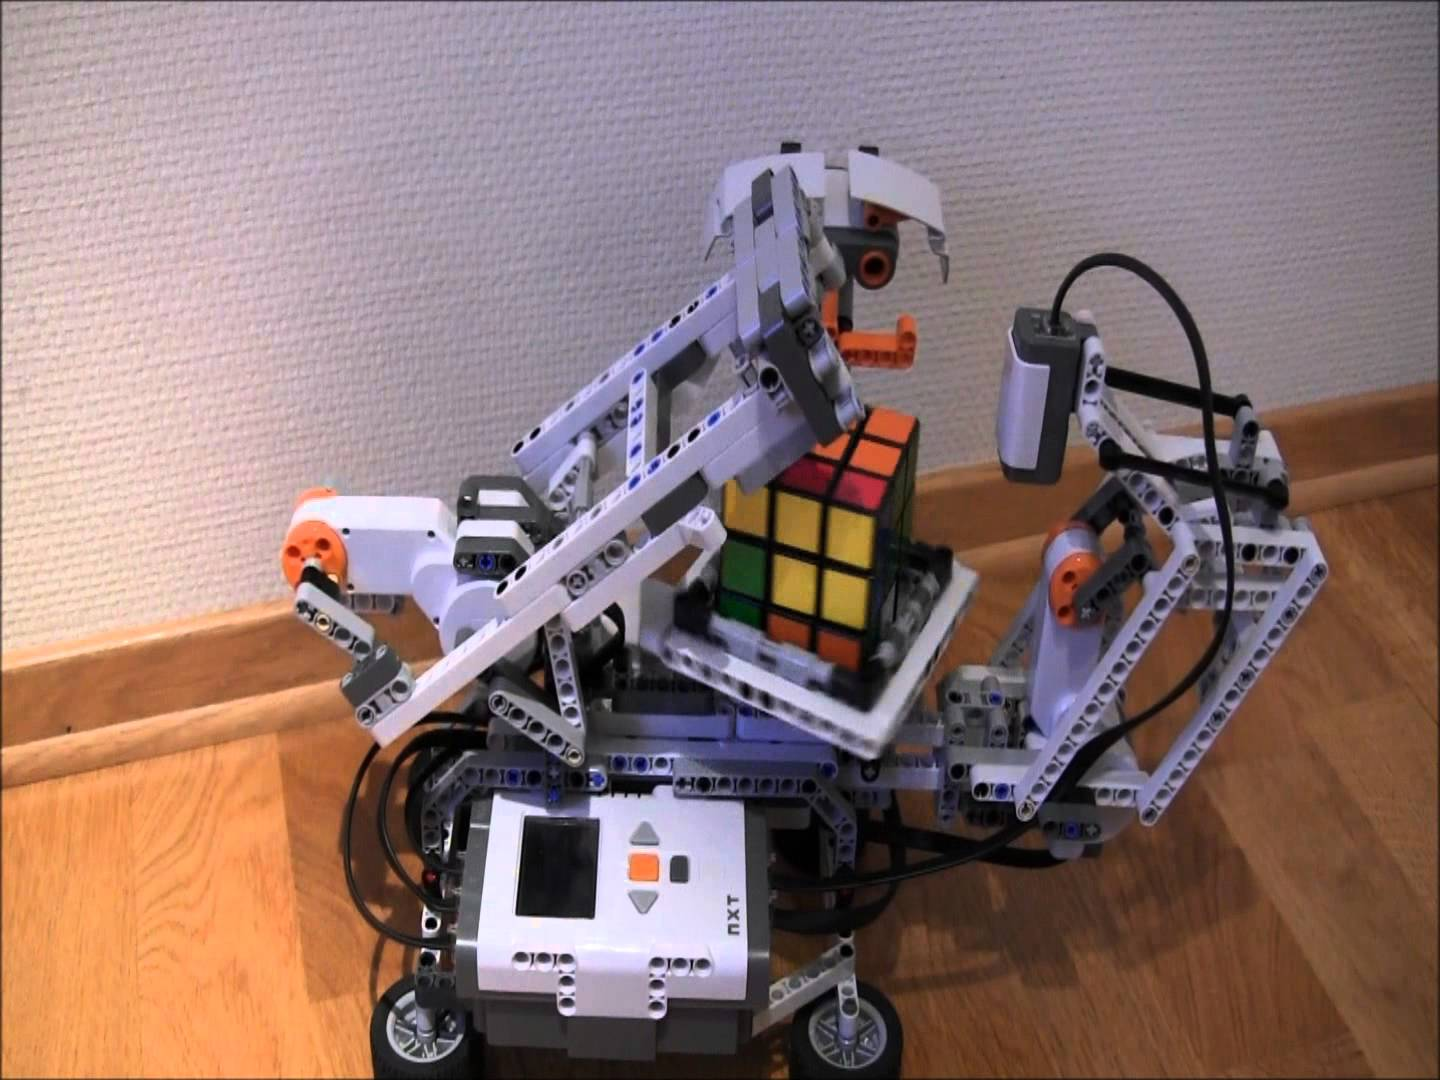
\includegraphics[width=0.3\linewidth]{images/prop1.jpg}
	\caption{Robot hecho con Lego} \label{fig:prop1}
\end{figure}
La propuesta de 8 motores fue descartada en su mayoría por la complejidad con la cual se había construido,
\begin{figure}[hb]
	\centering
	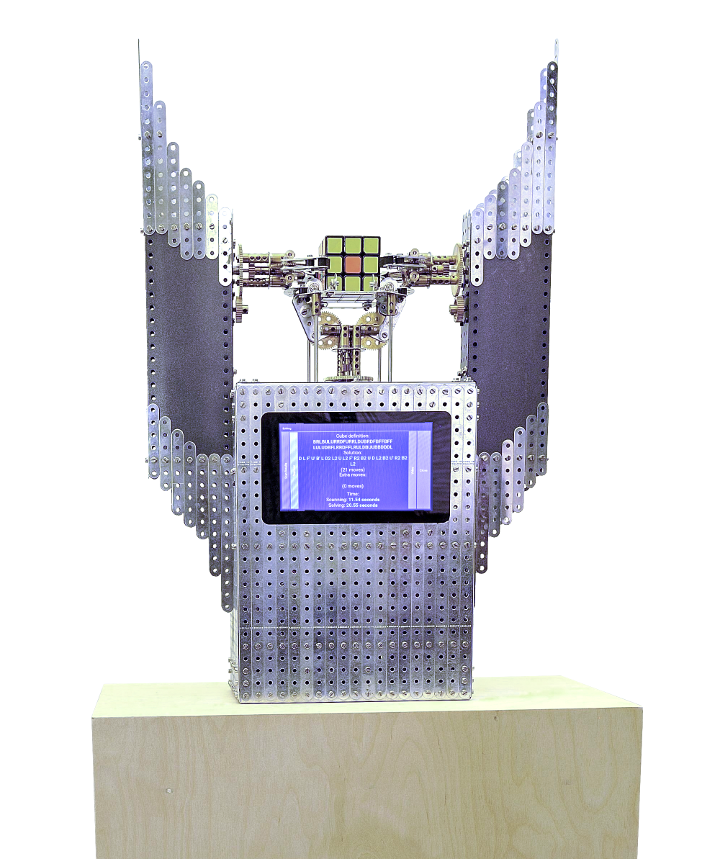
\includegraphics[width=0.3\linewidth]{images/prop2.png}
	\caption{Meccano Rubik's Shrine} \label{fig:prop1}
\end{figure}
\paragraph{}

\subsection{Análisis de soluciones.}
\subsection{Diseño}
\end{document}